\section{Basic}
\subsection{vimrc}
\lstinputlisting{01_Basic/.vimrc}
\subsection{Default code}
\lstinputlisting{01_Basic/default_code.cpp}
\subsection{readchar}
\lstinputlisting{01_Basic/readchar.cpp}
\subsection{readint}
\lstinputlisting{01_Basic/readint.cpp}
\subsection{Black Magic}
\lstinputlisting{01_Basic/black_magic.cpp}

\section{Graph}
\subsection{BCC Vertex*} % test by CF 102512 A
\lstinputlisting{02_Graph/BCC_Vertex.cpp}
\subsection{Bridge*} % test by TIOJ 1879
\lstinputlisting{02_Graph/Bridge.cpp}
\subsection{Bipartite Matching*} % test by TIOJ 1879
\lstinputlisting{02_Graph/Bipartite_Matching.cpp}
\subsection{2SAT (SCC)*} % SCC test by TIOJ 2143, 2SAT test by ARC069 F
\lstinputlisting{02_Graph/2SAT.cpp}
\subsection{MinimumMeanCycle*} % test by TIOJ 1934
\lstinputlisting{02_Graph/MinimumMeanCycle.cpp}
\subsection{Maximum Clique Dyn*} % test by TIOJ 1978
\lstinputlisting{02_Graph/Maximum_Clique_Dyn.cpp} 
\subsection{Maximum Clique*} % test by TIOJ 1978
\lstinputlisting{02_Graph/Maximum_Clique.cpp}
\subsection{Minimum Steiner Tree*} % test by luogu P6192
\lstinputlisting{02_Graph/MinimumSteinerTree.cpp}
\subsection{Minimum Arborescence*} % test by NTUJ 2176
\lstinputlisting{02_Graph/Minimum_Arborescence.cpp}
\subsection{Vizing's theorem}
\lstinputlisting{02_Graph/Vizing.cpp}
\subsection{Minimum Clique Cover*} % test by TIOJ 1472
\lstinputlisting{02_Graph/Minimum_Clique_Cover.cpp}
\subsection{NumberofMaximalClique*} % test by POJ 2989
\lstinputlisting{02_Graph/NumberofMaximalClique.cpp}
\subsection{Dijkstra*}
\lstinputlisting{02_Graph/Dijkstra.cpp}
\subsection{Kosaraju*}
\lstinputlisting{02_Graph/Kosaraju.cpp}
\subsection{Simple Graph Matching*}
\lstinputlisting{02_Graph/Simple_Graph_Matching.cpp}
\subsection{Two Edge Connected Components}
\lstinputlisting{02_Graph/Two_Edge_connected_components.cpp}
\subsection{Theory}
\begin{footnotesize}
$|$Maximum independent edge set$|=|V|-|$Minimum edge cover$|$\\
$|$Maximum independent set$|=|V|-|$Minimum vertex cover$|$\\
\end{footnotesize}
\subsection{LCA*}
\lstinputlisting{02_Graph/LCA.cpp}
\subsection{Tree Flatten*}
\lstinputlisting{02_Graph/Tree_Flatten.cpp}


\section{Data Structure}
\subsection{Leftist Tree}
\lstinputlisting{03_Data_Structure/Leftist_Tree.cpp}
\subsection{Heavy light Decomposition}
\lstinputlisting{03_Data_Structure/Heavy_light_Decomposition.cpp}
\subsection{Centroid Decomposition*} % test by TIOJ 1171
\lstinputlisting{03_Data_Structure/Centroid_Decomposition.cpp}
\subsection{Smart Pointer*}
\lstinputlisting{03_Data_Structure/Smart_Pointer.cpp}
\subsection{LiChaoST*}
\lstinputlisting{03_Data_Structure/LiChaoST.cpp}
\subsection{LiChaoSTSeg*}
\lstinputlisting{03_Data_Structure/LiChaoSTSeg.cpp}
\subsection{Link cut tree*} % test by luogu P3690
\lstinputlisting{03_Data_Structure/link_cut_tree.cpp}
\subsection{KDTree}
\lstinputlisting{03_Data_Structure/KDTree.cpp}
\subsection{Segment Tree with tag}
\lstinputlisting{03_Data_Structure/Segment_Tree_with_tag.cpp}
\subsection{2D Binary Indexed Tree}
\lstinputlisting{03_Data_Structure/2D_Binary_Indexed_Tree.cpp}


\section{Flow/Matching}
\subsection{Dinic}
\lstinputlisting{04_Flow_Matching/Dinic.cpp}
% \subsection{Kuhn Munkres}
% \lstinputlisting{04_Flow_Matching/Kuhn_Munkres.cpp}
% \subsection{MincostMaxflow}
% \lstinputlisting{04_Flow_Matching/MincostMaxflow.cpp}
% \subsection{Maximum Simple Graph Matching*} % test by TIOJ 1504
% \lstinputlisting{04_Flow_Matching/Maximum_Simple_Graph_Matching.cpp}
% \subsection{Minimum Weight Matching (Clique version)*} % test by uoj.ac 81
% \lstinputlisting{04_Flow_Matching/Minimum_Weight_Matching.cpp}
% \subsection{SW-mincut}
% \lstinputlisting{04_Flow_Matching/SW-mincut.cpp}
% \subsection{BoundedFlow(Dinic*)} % test by NTUJ 184(Only Dinic)
% \lstinputlisting{04_Flow_Matching/BoundedFlow.cpp}
% \subsection{Flow Models}
% \input{04_Flow_Matching/Model.tex}
% \subsection{isap}
% \lstinputlisting{04_Flow_Matching/isap.cpp}


\section{String}
\subsection{KMP}
\lstinputlisting{05_String/KMP.cpp}
\subsection{Z-value}
\lstinputlisting{05_String/Z-value.cpp}
\subsection{Manacher*} % test by TIOJ 1276
\lstinputlisting{05_String/Manacher.cpp}
\subsection{SAIS*}
\lstinputlisting{05_String/SAIS.cpp}
\subsection{Aho-Corasick Automaton}
\lstinputlisting{05_String/Aho-Corasick_Automaton.cpp}
\subsection{Smallest Rotation}
\lstinputlisting{05_String/Smallest_Rotation.cpp}
\subsection{De Bruijn sequence*} % test by CF 102001 C
\lstinputlisting{05_String/De_Bruijn_sequence.cpp}
\subsection{SAM}
\lstinputlisting{05_String/SAM.cpp}
\subsection{PalTree}
\lstinputlisting{05_String/PalTree.cpp}
\subsection{cyclicLCS}
\lstinputlisting{05_String/cyclicLCS.cpp}
\subsection{Suffix Array}
\lstinputlisting{05_String/Suffix_Array.cpp}
\subsection{Suffix Array2}
\lstinputlisting{05_String/Suffix_Array2.cpp}


\section{Math}
\subsection{exgcd*} % test by NTUJ 110
\lstinputlisting{06_Math/exgcd.cpp}
\subsection{floor and ceil}
\lstinputlisting{06_Math/floor_ceil.cpp}
\subsection{SG value}
\lstinputlisting{06_Math/SG_value.cpp}
% \subsection{floor sum*} % test by AtCoder Library Practice Contest C, CF 100920 J
% \lstinputlisting{06_Math/floor_sum.cpp}
\subsection{Miller Rabin*} % test by NTUJ 1237
\lstinputlisting{06_Math/Miller_Rabin.cpp}
\subsection{Big number}
\lstinputlisting{06_Math/Big_number.cpp}
\subsection{Fraction}
\lstinputlisting{06_Math/Fraction.cpp}
\subsection{Simultaneous Equations}
\lstinputlisting{06_Math/Simultaneous_Equations.cpp}
\subsection{Pollard Rho}
\lstinputlisting{06_Math/Pollard_Rho.cpp}
\subsection{Simplex Algorithm}
\lstinputlisting{06_Math/Simplex_Algorithm.cpp}
\subsubsection{Construction}
\input{06_Math/SimplexConstruction.tex}
\subsection{Schreier-Sims Algorithm*} % test by XVI Opencup GP of Ekaterinburg H
\lstinputlisting{06_Math/SchreierSims.cpp}
\subsection{chineseRemainder}
\lstinputlisting{06_Math/chineseRemainder.cpp}
\subsection{QuadraticResidue}
\lstinputlisting{06_Math/QuadraticResidue.cpp}
\subsection{Discrete Log}
\lstinputlisting{06_Math/DiscreteLog.cpp}
\subsection{PiCount}
\lstinputlisting{06_Math/PiCount.cpp}
\subsection{Primes}
\lstinputlisting{06_Math/Primes.cpp}
\subsection{Mod Sqrt}
\lstinputlisting{06_Math/modsqrt.cpp}
\subsection{Theorem}
\input{06_Math/Theorem.tex}
\subsection{Euclidean Algorithms}
\input{06_Math/Euclidean.tex}

\section{Polynomial}
\subsection{Fast Fourier Transform}
\lstinputlisting{07_Polynomial/Fast_Fourier_Transform.cpp}
\subsection{Number Theory Transform}
\lstinputlisting{07_Polynomial/Number_Theory_Transform.cpp}
\subsection{Fast Walsh Transform*} % test by luogu P6097
\lstinputlisting{07_Polynomial/Fast_Walsh_Transform.cpp}
%\subsection{Polynomial Operation}
%\lstinputlisting{07_Polynomial/Polynomial_Operation.cpp}
\subsection{Newton's Method}
\input{07_Polynomial/Newton.tex}

\section{Geometry}
\subsection{Default Code}
\lstinputlisting{08_Geometry/Default_code.cpp}
\subsection{Convex hull*} % test by Zerojudge b398
\lstinputlisting{08_Geometry/Convex_hull.cpp}
\subsection{External bisector}
\lstinputlisting{08_Geometry/external_bisector.cpp}
\subsection{Heart}
\lstinputlisting{08_Geometry/Heart.cpp}
\subsection{Minimum Enclosing Circle*} % test by TIOJ 1093
\lstinputlisting{08_Geometry/Minimum_Enclosing_Circle.cpp}
\subsection{Polar Angle Sort*} % test by NTUJ 2270
\lstinputlisting{08_Geometry/Polar_Angle_Sort.cpp}
\subsection{Intersection of two circles*} % test by TIOJ 1503
\lstinputlisting{08_Geometry/Intersection_of_two_circles.cpp}
\subsection{Intersection of polygon and circle}
\lstinputlisting{08_Geometry/Intersection_of_polygon_and_circle.cpp}
\subsection{Intersection of line and circle}
\lstinputlisting{08_Geometry/Intersection_of_line_and_circle.cpp}
\subsection{point in circle}
\lstinputlisting{08_Geometry/point_in_circle.cpp}
\subsection{Half plane intersection}
\lstinputlisting{08_Geometry/Half_plane_intersection.cpp}
\subsection{CircleCover*} % test by TIOJ 1503
\lstinputlisting{08_Geometry/CircleCover.cpp}
\subsection{3Dpoint*} % test by HDU 3662
\lstinputlisting{08_Geometry/3Dpoint.cpp}
\subsection{Convexhull3D*} % test by HDU 3662
\lstinputlisting{08_Geometry/Convexhull3D.cpp}
\subsection{Tangent line of two circles}
\lstinputlisting{08_Geometry/Tangent_line_of_two_circles.cpp}
\subsection{minMaxEnclosingRectangle}
\lstinputlisting{08_Geometry/minMaxEnclosingRectangle.cpp}
\subsection{minDistOfTwoConvex}
\lstinputlisting{08_Geometry/minDistOfTwoConvex.cpp}
\subsection{Minkowski Sum*} % test by Zerojudge b398
\lstinputlisting{08_Geometry/Minkowski_Sum.cpp}
\subsection{RotatingSweepLine}
\lstinputlisting{08_Geometry/rotatingSweepLine.cpp}

\section{Else}
% \subsection{Mo's Alogrithm(With modification)}
% \lstinputlisting{09_Else/Mos_Alogrithm_With_modification.cpp}
% \subsection{Mo's Alogrithm On Tree}
% \lstinputlisting{09_Else/Mos_Alogrithm_On_Tree.cpp}
% \subsection{DynamicConvexTrick*} % test by TIOJ 1921
% \lstinputlisting{09_Else/DynamicConvexTrick.cpp}
% \subsection{DLX*} % test by TIOJ 1333, 1381
% \lstinputlisting{09_Else/DLX.cpp}
% \subsection{Matroid Intersection}
% \input{09_Else/Matroid.tex}
% \subsection{AdaptiveSimpson}
% \lstinputlisting{09_Else/AdaptiveSimpson.cpp}
\subsection{Closest Pair}
\lstinputlisting{09_Else/Closest_Pair.cpp}


\newpage
\onecolumn
\noindent
\centering
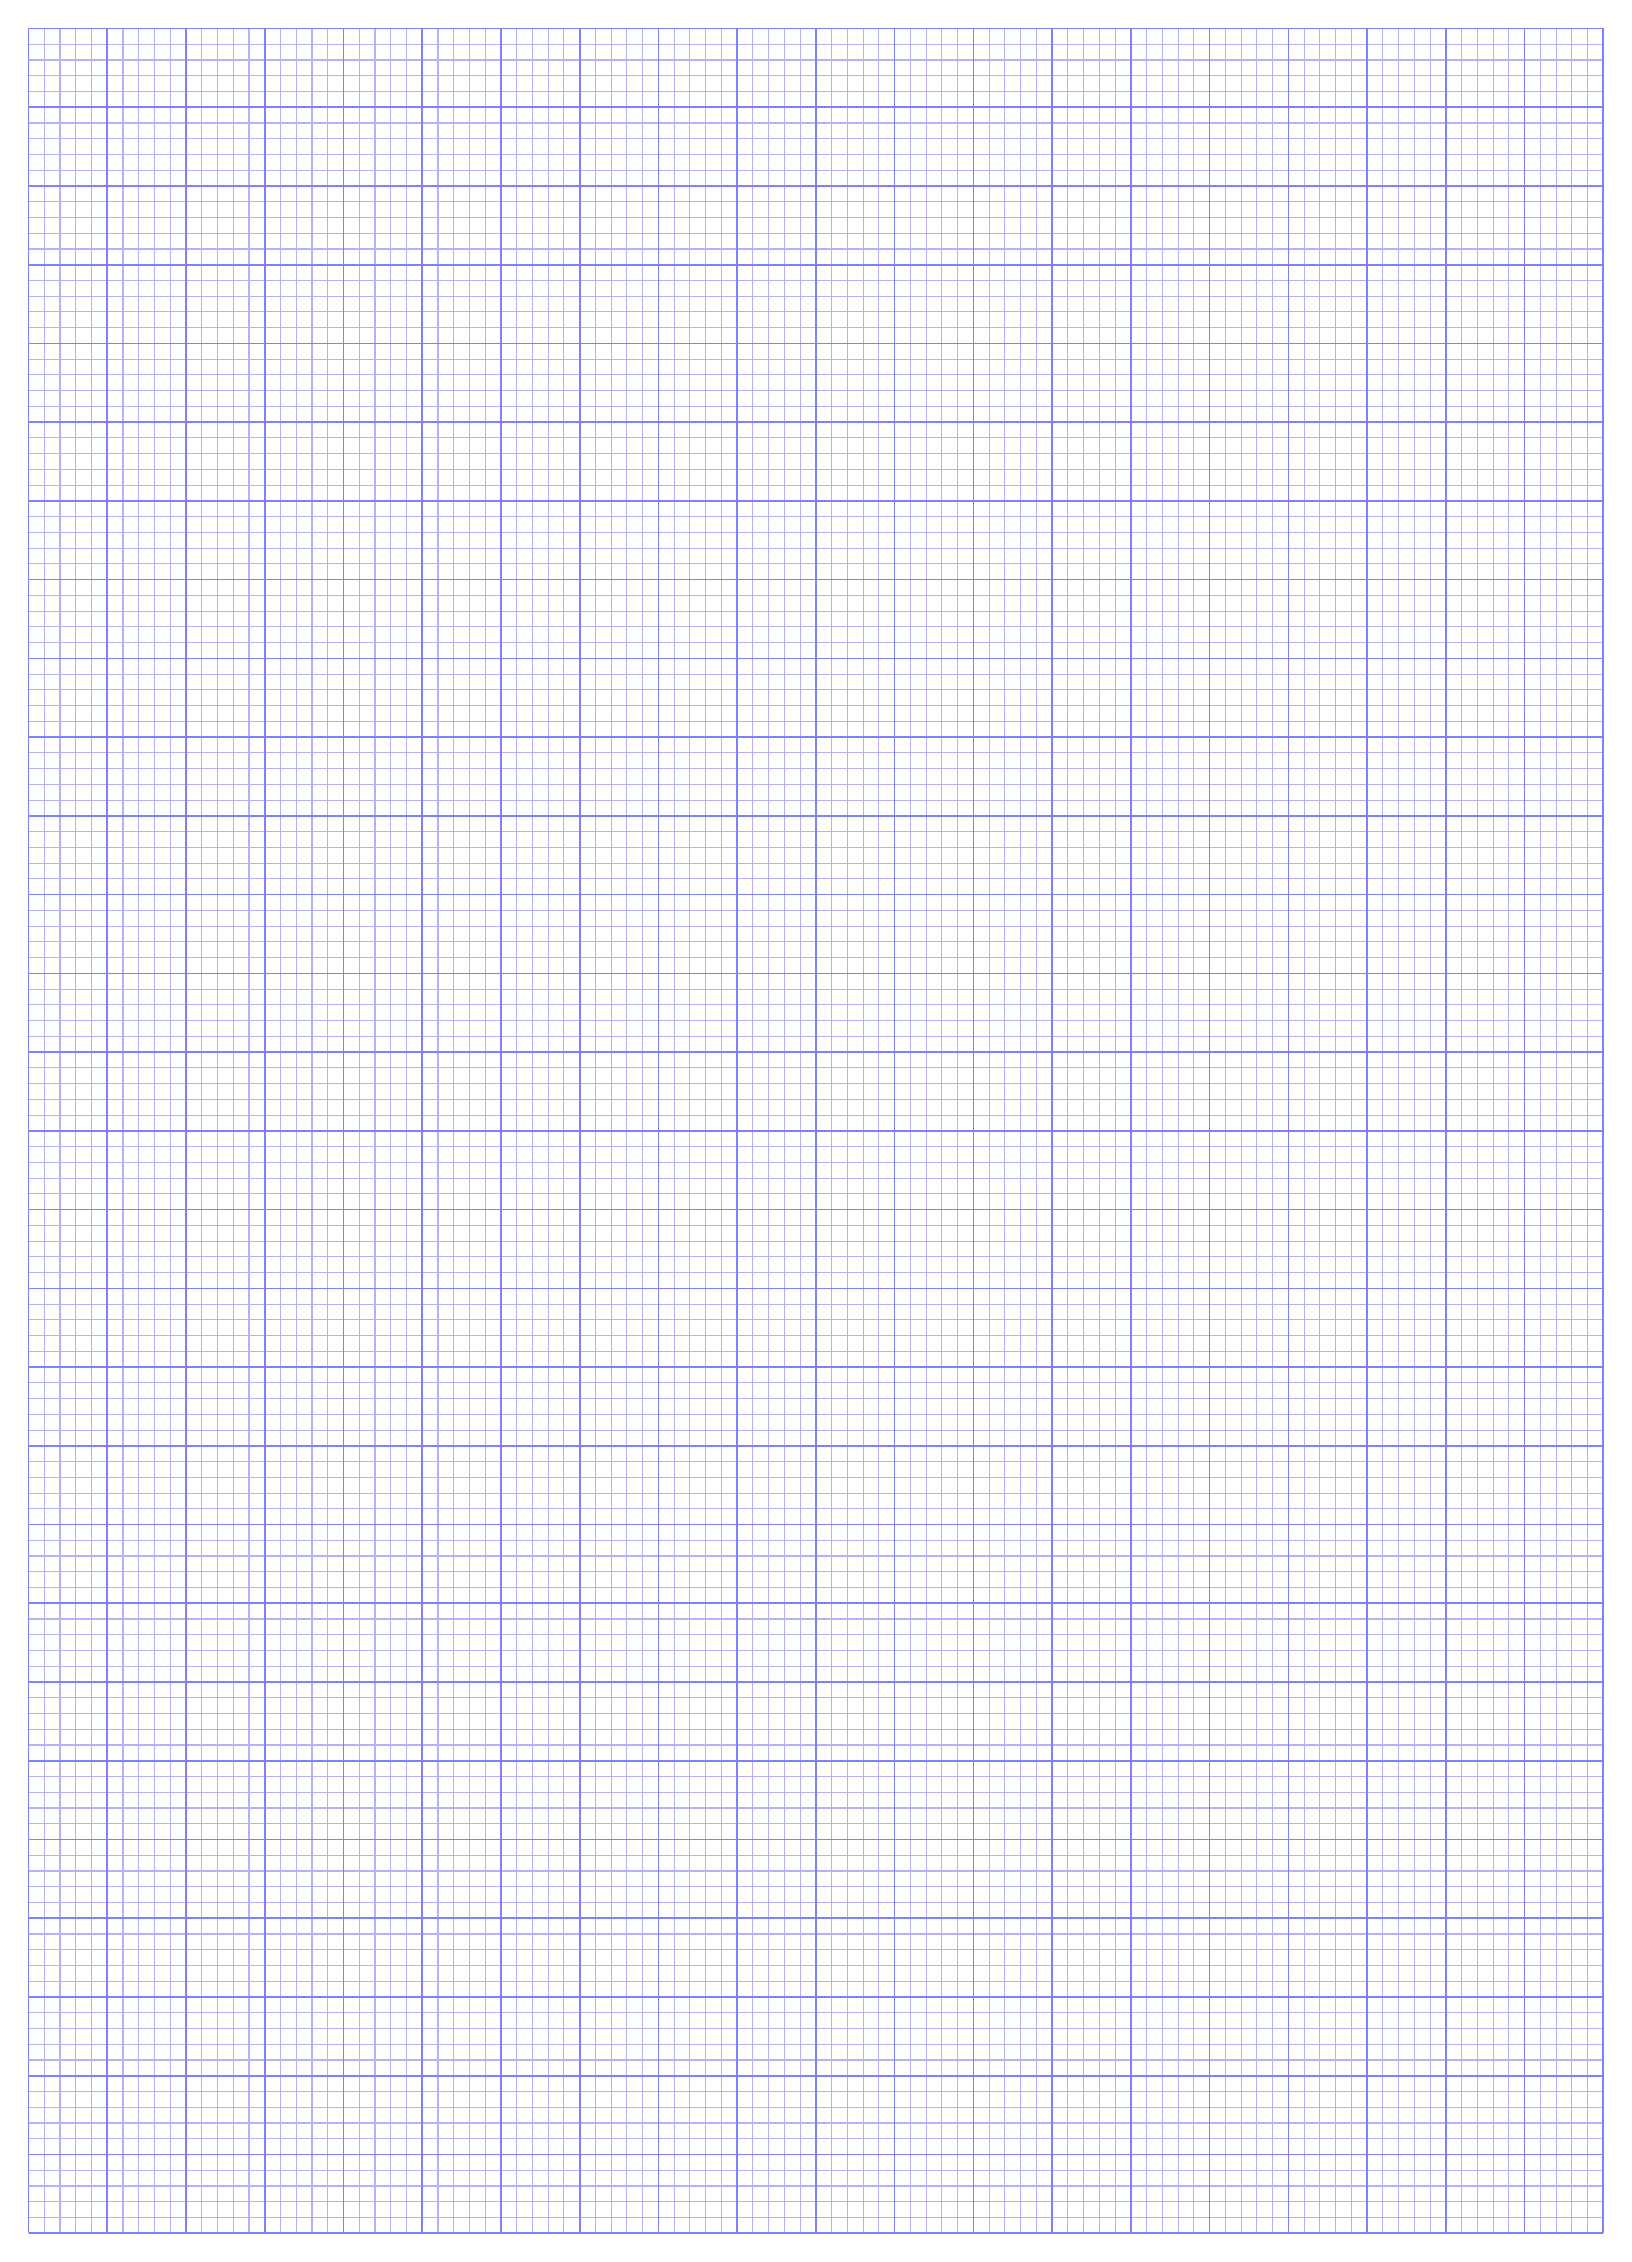
\begin{tikzpicture}
% \draw[blue,very thin](0,0)grid[step=0.5cm](6.5,10);
\draw[line width=.4pt,draw=blue!30] (0,0) grid[step=2mm] (20,28);
\draw[line width=.6pt,draw=blue!50] (0,0) grid[step=1cm] (20,28);
\end{tikzpicture}
